% This is sigproc-sp.tex -FILE FOR V2.6SP OF ACM_PROC_ARTICLE-SP.CLS
% OCTOBER 2002
%
% It is an example file showing how to use the 'acm_proc_article-sp.cls' V2.6SP
% LaTeX2e document class file for Conference Proceedings submissions.
% ----------------------------------------------------------------------------------------------------------------
% This .tex file (and associated .cls V2.6SP) *DOES NOT* produce:
%       1) The Permission Statement
%       2) The Conference (location) Info information
%       3) The Copyright Line with ACM data
%       4) Page numbering
%
%  However, both the CopyrightYear (default to 2002) and the ACM Copyright Data
% (default to X-XXXXX-XX-X/XX/XX) can still be over-ridden by whatever the author
% inserts into the source .tex file.
% e.g.
% \CopyrightYear{2003} will cause 2003 to appear in the copyright line.
% \crdata{0-12345-67-8/90/12} will cause 0-12345-67-8/90/12 to appear in the copyright line.
%
% ---------------------------------------------------------------------------------------------------------------
% It is an example which *does* use the .bib file (from which the .bbl file
% is produced).
% REMEMBER HOWEVER: After having produced the .bbl file,
% and prior to final submission,
% you need to 'insert'  your .bbl file into your source .tex file so as to provide
% ONE 'self-contained' source file.
%
% Questions regarding SIGS should be sent to
% Adrienne Griscti ---> griscti@acm.org
%
% Questions/suggestions regarding the guidelines, .tex and .cls files, etc. to
% Gerald Murray ---> murray@acm.org
%
% For tracking purposes - this is V2.6SP - OCTOBER 2002

\documentclass{acm_proc_article-sp-sigmod09}
\usepackage{url}
\begin{document}
%
% --- Author Metadata here ---
\conferenceinfo{Big Data and Social Networks}{Academic year 2018-2019}
%\setpagenumber{50}
%\CopyrightYear{2002} % Allows default copyright year (2002) to be over-ridden - IF NEED BE.
%\crdata{0-12345-67-8/90/01}  % Allows default copyright data (X-XXXXX-XX-X/XX/XX) to be over-ridden.
% --- End of Author Metadata ---

\title{A data generator for frequent itemset mining in tree-like sequences of complex objects \\ \large Nicol\`o Pomini [203319] and Marco Merlin[205263]}
%
% You need the command \numberofauthors to handle the "boxing"
% and alignment of the authors under the title, and to add
% a section for authors number 4 through n.

\numberofauthors{2}
%
\maketitle
\begin{abstract}
Data generation is essential to many companies nowadays, allowing testing data mining and processing applications using an almost unlimited amounts of data without being forced to buy it from third party businesses. While it is often true that generated data cannot have the same quality as real world data, it can still come pretty close by using parameterized generators, which can vary the generated data based on some parameters dictated by the user. In this way it is possible to change the way the data is generated, and so to simulate different real world scenarios. In the next chapters are described the algorithms, the methods used and the results obtained by developing a parameterized data generator for frequent itemsets in tree-like sequences of complex objects. Tree structures formed by complex objects are generated with dependencies between their attributes, meaning that the same sequence of attributes appears frequently in the generated trees. The generator uses different parameters to generate different patterns and change the way attributes depend from each other, so that many scenarios can be simulated. Further details about all the possible parameters can be found in the next chapters.
\end{abstract}

\terms{Data mining}

\keywords{Data generation, frequent itemset mining}

\section{Introduction}
Nowadays, the daily generation of data is growing exponentially. People, companies, sensors, IoT devices and many other things produce every day a huge amount of data: according to forbes.com\footnote{forbes.com/sites/bernardmarr/2018/05/21/how-much-data-do-we-create-every-day-the-mind-blowing-stats-everyone-should-read}, 2.5 quintillion bytes of data are generates. Thanks to these numbers, several fields of computer science related to data are also growing very fast. One of these is \emph{data mining}.

As suggested by its name, the aim of data mining is to discover and extract pattern, and more general information, from great amount of data. The larger the available dataset, the more accurate and meaningful the results. Data mining involves many techniques, which are coming not only from the computer science area, such as statistics and data visualization. 

One possible field of data mining is the frequent itemset mining. In many scenarios, applications produce records that contain several fields, and these fields are not always indepentent, but the appearence of one may mean the appearence of some others. For example, a list of purchases in a shop can contain similar patterns, or a call made by a web service to some external RESTful services may lead to further calls to other services.

This report is about the project for the \emph{Big Data and Social networks} course offered by the department of information engineering and computer science\footnote{\url{www.disi.unitn.it}} of the university of Trento. The project is related to the \emph{data mining} course, offered by the same department, and in particular to the course project of the latter. In fact, the purpose of the \emph{big data} project is to build a data generator for the \emph{data mining} project.

The report is organized as follows: in Chapter 2, the problem statement is formalized, \dots.

\section{Problem statement}
The goal of this project is to create a data generator for the \emph{data mining} project. To better understand which are the constraints to consider, let us formalize the \emph{data mining} problem.

\subsection{Data mining problem statement}
A record $\boldsymbol{r}$ is a tuple, in the form $<a_1 \colon v_1, a_2 \colon v_2, \text{\dots}, a_n \colon v_n>$, where a pair $a_i \colon v_i$ represents is a attribute-value relationship, where $a_i$ is the attribute and $v_i$ the value. These pairs can contain any kind of data, such as numbers or strings. To identify a record, is assumed that each one has an attribute called \emph{record id}, or \texttt{rid} for short.

A transaction $\boldsymbol{T}$ is a set of records $\{\boldsymbol{r_1}, \boldsymbol{r_2}, \text{\dots}, \boldsymbol{r_m}\}$ that forms a tree structure, which means that a transaction has a root record, which has some \emph{children records}, which in turn other children, and so on. To identify the transaction in which each record belongs, it is assumed that every record has an attribute called \emph{transaction id}, or \texttt{tid} for short.

\begin{figure}
\centering
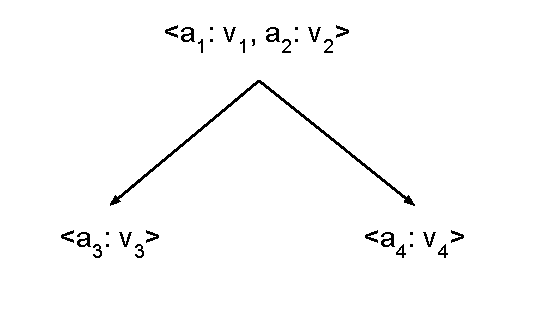
\epsfig{file=PatternExample.pdf}
\caption{An example of transaction, made of three records.}
\label{fig:transaction}
\end{figure}

A pattern is a set of ordered attributes and values belonging to possibly different records in the same transaction. In other words, a pattern is any ordered subset of $\bigcup\limits_{i=1}^{n} \bigcup\limits_{j=1}^{m} \boldsymbol{r_i}<a_j \colon v_j>$, where the ordering is given by the hierarchy of the transaction. For example, in Figure~\ref{fig:transaction} some possible example of pattern are $\{a_1 \colon v_1, a_3 \colon v_3\}$ or $\{a_2 \colon v_2, a_3 \colon v_3\}$, but not $\{a_4 \colon v_4, a_1 \colon v_1\}$, beacuse the latter breakes the hierarchic order.

Given a set of transactions, the goal is to identify patterns of attributes that are frequent, which means transaction that appear at least a given number of time $f$.

\subsection{Big Data problem}
Starting from the data mining problem statement, the big data one is to create a set of records, which are organized in tree-structured transactions, making sure that among the transactions there exist some frequent pattern.

\section{Assumptions}
For the sake of simplification, some assumption exists.

All the records contain at least three attributes: the \texttt{rid} to identify the record, the \texttt{tid} to recognize to which transaction the record belongs, and a \texttt{parent} field, containing the \texttt{rid} of the parent record -- which can be empty in case the considered record is the root of a transaction.

All the records are assumed to have the same attributes -- some of them may be empty. Each record has discrete values, belonging to finite sets of possible values. This assumption is needed to make the data mining project easier. From the point of view of the data generation, the absence of this constraint would not complicate anything.

\subsection{Math Equations}
You may want to display math equations in three distinct styles:
inline, numbered or non-numbered display.  Each of
the three are discussed in the next sections.

\subsubsection{Inline (In-text) Equations}
A formula that appears in the running text is called an
inline or in-text formula.  It is produced by the
\textbf{math} environment, which can be
invoked with the usual \texttt{{\char'134}begin. . .{\char'134}end}
construction or with the short form \texttt{\$. . .\$}. You
can use any of the symbols and structures,
from $\alpha$ to $\omega$, available in
\LaTeX\cite{Lamport:LaTeX}; this section will simply show a
few examples of in-text equations in context. Notice how
this equation: \begin{math}\lim_{n\rightarrow \infty}x=0\end{math},
set here in in-line math style, looks slightly different when
set in display style.  (See next section).

\subsubsection{Display Equations}
A numbered display equation -- one set off by vertical space
from the text and centered horizontally -- is produced
by the \textbf{equation} environment. An unnumbered display
equation is produced by the \textbf{displaymath} environment.

Again, in either environment, you can use any of the symbols
and structures available in \LaTeX; this section will just
give a couple of examples of display equations in context.
First, consider the equation, shown as an inline equation above:
\begin{equation}\lim_{n\rightarrow \infty}x=0\end{equation}
Notice how it is formatted somewhat differently in
the \textbf{displaymath}
environment.  Now, we'll enter an unnumbered equation:
\begin{displaymath}\sum_{i=0}^{\infty} x + 1\end{displaymath}
and follow it with another numbered equation:
\begin{equation}\sum_{i=0}^{\infty}x_i=\int_{0}^{\pi+2} f\end{equation}
just to demonstrate \LaTeX's able handling of numbering.

\subsection{Tables}
Because tables cannot be split across pages, the best
placement for them is typically the top of the page
nearest their initial cite.  To
ensure this proper ``floating'' placement of tables, use the
environment \textbf{table} to enclose the table's contents and
the table caption.  The contents of the table itself must go
in the \textbf{tabular} environment, to
be aligned properly in rows and columns, with the desired
horizontal and vertical rules.  Again, detailed instructions
on \textbf{tabular} material
is found in the \textit{\LaTeX\ User's Guide}.

Immediately following this sentence is the point at which
Table 1 is included in the input file; compare the
placement of the table here with the table in the printed
dvi output of this document.

\begin{table}
\centering
\caption{Frequency of Special Characters}
\begin{tabular}{|c|c|l|} \hline
Non-English or Math&Frequency&Comments\\ \hline
\O & 1 in 1,000& For Swedish names\\ \hline
$\pi$ & 1 in 5& Common in math\\ \hline
\$ & 4 in 5 & Used in business\\ \hline
$\Psi^2_1$ & 1 in 40,000& Unexplained usage\\
\hline\end{tabular}
\end{table}

To set a wider table, which takes up the whole width of
the page's live area, use the environment
\textbf{table*} to enclose the table's contents and
the table caption.  As with a single-column table, this wide
table will ``float" to a location deemed more desirable.
Immediately following this sentence is the point at which
Table 2 is included in the input file; again, it is
instructive to compare the placement of the
table here with the table in the printed dvi
output of this document.


\begin{table*}
\centering
\caption{Some Typical Commands}
\begin{tabular}{|c|c|l|} \hline
Command&A Number&Comments\\ \hline
\texttt{{\char'134}alignauthor} & 100& Author alignment\\ \hline
\texttt{{\char'134}numberofauthors}& 200& Author enumeration\\ \hline
\texttt{{\char'134}table}& 300 & For tables\\ \hline
\texttt{{\char'134}table*}& 400& For wider tables\\ \hline\end{tabular}
\end{table*}
% end the environment with {table*}, NOTE not {table}!

As was the case with tables, you may want a figure
that spans two columns.  To do this, and still to
ensure proper ``floating'' placement of tables, use the environment
\textbf{figure*} to enclose the figure and its caption.
\begin{figure*}
\centering
\epsfig{file=flies.eps}
\caption{A sample black and white graphic (.eps format)
that needs to span two columns of text.}
\end{figure*}
and don't forget to end the environment with
{figure*}, not {figure}!

\subsection{Theorem-like Constructs}
Other common constructs that may occur in your article are
the forms for logical constructs like theorems, axioms,
corollaries and proofs.  There are
two forms, one produced by the
command \texttt{{\char'134}newtheorem} and the
other by the command \texttt{{\char'134}newdef}; perhaps
the clearest and easiest way to distinguish them is
to compare the two in the output of this sample document:

This uses the \textbf{theorem} environment, created by
the \texttt{{\char'134}newtheorem} command:
\newtheorem{theorem}{Theorem}
\begin{theorem}
Let $f$ be continuous on $[a,b]$.  If $G$ is
an antiderivative for $f$ on $[a,b]$, then
\begin{displaymath}\int^b_af(t)dt = G(b) - G(a).\end{displaymath}
\end{theorem}

The other uses the \textbf{definition} environment, created
by the \texttt{{\char'134}newdef} command:
\newdef{definition}{Definition}
\begin{definition}
If $z$ is irrational, then by $e^z$ we mean the
unique number which has
logarithm $z$: \begin{displaymath}{\log e^z = z}\end{displaymath}
\end{definition}

Two lists of constructs that use one of these
forms is given in the
\textit{Author's  Guidelines}.

There is one other similar construct environment, which is
already set up
for you; i.e. you must \textit{not} use
a \texttt{{\char'134}newdef} command to
create it: the \textbf{proof} environment.  Here
is a example of its use:
\begin{proof}
Suppose on the contrary there exists a real number $L$ such that
\begin{displaymath}
\lim_{x\rightarrow\infty} \frac{f(x)}{g(x)} = L.
\end{displaymath}
Then
\begin{displaymath}
l=\lim_{x\rightarrow c} f(x)
= \lim_{x\rightarrow c}
\left[ g{x} \cdot \frac{f(x)}{g(x)} \right ]
= \lim_{x\rightarrow c} g(x) \cdot \lim_{x\rightarrow c}
\frac{f(x)}{g(x)} = 0\cdot L = 0,
\end{displaymath}
which contradicts our assumption that $l\neq 0$.
\end{proof}

\section{Conclusions}
This paragraph will end the body of this sample document.
Remember that you might still have Acknowledgments or
Appendices; brief samples of these
follow.  There is still the Bibliography to deal with; and
we will make a disclaimer about that here: with the exception
of the reference to the \LaTeX\ book, the citations in
this paper are to articles which have nothing to
do with the present subject and are used as
examples only.
%\end{document}  % This is where a 'short' article might terminate
%
% The following two commands are all you need in the
% initial runs of your .tex file to
% produce the bibliography for the citations in your paper.
\bibliographystyle{abbrv}
\bibliography{sigproc}  % sigproc.bib is the name of the Bibliography in this case
% You must have a proper ".bib" file
%  and remember to run:
% latex bibtex latex latex
% to resolve all references
%
% ACM needs 'a single self-contained file'!
%
%APPENDICES are optional
%\balancecolumns
\appendix
%Appendix A
\section{Headings in Appendices}
The rules about hierarchical headings discussed above for
the body of the article are different in the appendices.
In the \textbf{appendix} environment, the command
\textbf{section} is used to
indicate the start of each Appendix, with alphabetic order
designation (i.e. the first is A, the second B, etc.) and
a title (if you include one).  So, if you need
hierarchical structure
\textit{within} an Appendix, start with \textbf{subsection} as the
highest level. Here is an outline of the body of this
document in Appendix-appropriate form:
\subsection{Introduction}
\subsection{The Body of the Paper}
\subsubsection{Type Changes and  Special Characters}
\subsubsection{Math Equations}
\paragraph{Inline (In-text) Equations}
\paragraph{Display Equations}
\subsubsection{Citations}
\subsubsection{Tables}
\subsubsection{Figures}
\subsubsection{Theorem-like Constructs}
\subsubsection*{A Caveat for the \TeX\ Expert}
\subsection{Conclusions}
\subsection{Acknowledgments}
\subsection{Additional Authors}
This section is inserted by \LaTeX; you do not insert it.
You just add the names and information in the
\texttt{{\char'134}additionalauthors} command at the start
of the document.
\subsection{References}
Generated by bibtex from your ~.bib file.  Run latex,
then bibtex, then latex twice (to resolve references)
to create the ~.bbl file.  Insert that ~.bbl file into
the .tex source file and comment out
the command \texttt{{\char'134}thebibliography}.
% This next section command marks the start of
% Appendix B, and does not continue the present hierarchy
\section{More Help for the Hardy}
The acm\_proc\_article-sp document class file itself is chock-full of succinct
and helpful comments.  If you consider yourself a moderately
experienced to expert user of \LaTeX, you may find reading
it useful but please remember not to change it.

% That's all folks!
\end{document}
